\documentclass{article}
\usepackage{graphicx}
\usepackage{amsmath}
\usepackage{amsfonts}
\usepackage[italian]{babel}
\graphicspath{{/}}
\begin{document}
\section{Equazioni dello stato ed equilibrio}
\begin{figure}[h]
    \centering
    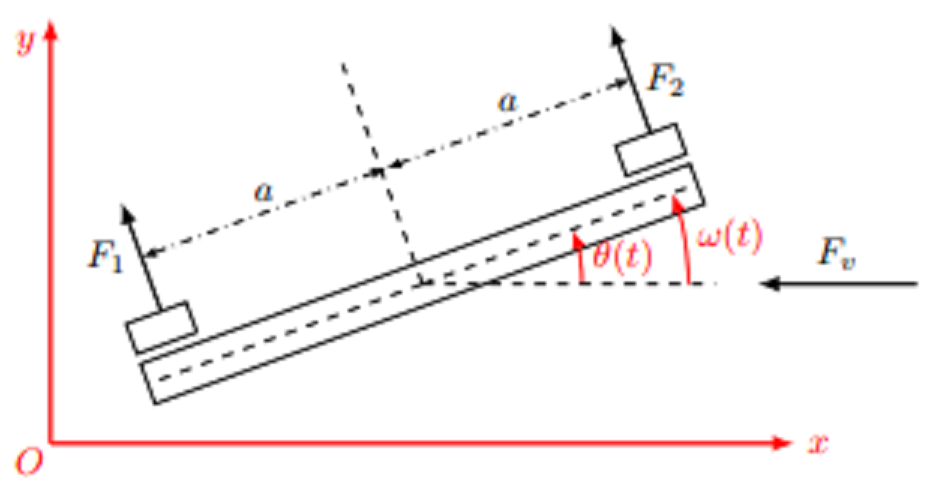
\includegraphics[width=0.75\textwidth]{figura drone}
    \caption{}
    \label{fig:drone}
\end{figure}
Equazioni dello stato:
\[u(t)=F_{p}\]
\[f(x(t),u(t))=\begin{bmatrix}
x_{2}(t)\\ \frac{ - \beta x_{2}(t) + \frac{a}{2}\sin{ (x_{1}(t)) } F_{v} + a u(t)} {J}
\end{bmatrix}\]
\[y(t)=h(x(t))=x_{1}(t)\]

Dove:
\begin{itemize}
\item $x(t)_{1}=y(t)=\theta(t)$ indica l'angolo di inclinazione rispetto al piano
\item $x(t)_{2}=\omega(t)$ indica la velocità di rotazione rispetto all'asse perpendicolare al \textit{piano passante per il baricentro}
\item $J$(param.) indica il momento di inerzia del drone rispetto all'asse di rotazione che passa per il baricentro
\item $\beta$(param.) indica il coefficiente d'attrito dinamico dovuto alla presenza dell'aria
\item $a$(parametro) indica la semi-ampiezza planare del drone
\item $F_{v}$(param.) indica la forza costante
dovuta all'azione del vento
\item $F_{p}(t)=F_{1}(t)-F_{2}(t)$ indica la differenza tra le forze
di propulsione $F_{1}(t)$ ed $F_{2}(t)$ applicate sul drone (come indicato in figura \ref{fig:drone})
\end{itemize} 

Considerando che:
\begin{itemize}
\item $J=10 \frac{kg}{m^2}$
\item $\beta=0.5 N$
\item $a=0.01 m$
\item $F_{v}=-5 N$
\item $\theta_{e}=\frac{\pi}{3} rad$
\end{itemize}


Per trovare la coppia di equilibrio poniamo $f(x(t),u(t))=0$, quindi
\[\begin{bmatrix}
x_{2}(t)\\ \frac{ - \beta x_{2}(t) + \frac{a}{2}\sin{ (x_{1}(t)) } F_{v} + a u(t)} {J}
\end{bmatrix}=0\]
\[\begin{bmatrix}
x_{2}(t)\\ \frac{\frac{0.01}{2}\sin{(\frac{\pi}{3})} (-5)+0.01u(t)}{10}
\end{bmatrix}=0 \]
\[\begin{bmatrix}
x_{2}(t)\\
\frac{\frac{-0.05\sqrt{3}}{2}+0.01u(t)}{10}
\end{bmatrix}=0 \]
\[\begin{bmatrix}
x_{2}(t)\\
\frac{-\sqrt{3}}{400}+\frac{u(t)}{1000}
\end{bmatrix}=0 \]
\[\begin{bmatrix}
x_{2}(t)\\
\frac{5}{2}\sqrt{3}
\end{bmatrix}=\begin{bmatrix}0\\u(t)\end{bmatrix} \]

Quindi la coppia di equilibrio è \[\left(\begin{bmatrix}
\frac{\pi}{3}
\\
0
\end{bmatrix}
,\frac{5}{2}\sin{\left(\frac{\pi}{3}\right)}=u_e=2.17\right)\]

\section{Linearizzazione della funzione nel punto di equilibrio}
Per linearizzare la funzione è necessario derivare la funzione per poi arrivare a \[\delta \dot{x}=A \delta x+B\delta u\]\[\delta \dot{y}=C \delta x + D \delta u\]


Calcoliamo la Jacobiana per f:
\[\begin{bmatrix}
\frac{\partial f_1}{\partial x_1} && \frac{\partial f_1}{\partial x_2} && \frac{\partial f_1}{\partial u}
\\
\frac{\partial f_2}{\partial x_1} && \frac{\partial f_2}{\partial x_2} && \frac{\partial f_2}{\partial u}
\end{bmatrix}\]
\[\begin{bmatrix}
0 && 1 && 0
\\
\frac{aF_{v}}{2J}\cos{(x_1(t))} && -\beta && a
\end{bmatrix}\]
E facciamo le derivate parziali per h:
\[\frac{\partial h}{\partial x}=\begin{bmatrix}
\frac{\partial h_1}{\partial x_1} && \frac{\partial h_1}{\partial x_2} \end{bmatrix}=\begin{bmatrix}
1 && 0 \end{bmatrix}\]
\[\frac{\partial h}{\partial u}=0\]
Che nell'equilibrio valgono:
\[\begin{bmatrix}
0 && 1 && 0
\\
\frac{aF_{v}}{2J}\cos{(x_{1e})} && -\frac{\beta}{J} && \frac{a}{J}
\end{bmatrix}\]
\[\begin{bmatrix}
1 && 0 \end{bmatrix}\]
\[0\]
Quindi:
\[A=\begin{bmatrix}
0 && 1
\\
\frac{aF_{v}}{2J}\cos{(x_{1e})} && -\frac{\beta}{J}
\end{bmatrix}\]
\[B=\begin{bmatrix}
0
\\
\frac{a}{J} 
\end{bmatrix}\]
\[C=\begin{bmatrix}
1 && 0 \end{bmatrix}\]
\[D=0\]
\section{Funzione di trasferimento}
La funzione di trasferimento viene calcolata secondo
\[G(s)=C(sI-A)^{-1}B+D\]
\end{document}
